\section{Datenbanktechnologie, Datenmodell und Umsetzung}

Für die Umsetzung einer generischen, datenmodellgesteuerten Erweiterung wurde ein flexibles und zur Laufzeit auswertbares Schema benötigt. Anstelle eines statisch implementierten Modells basiert die Lösung auf einer dynamischen Analyse eines zentral definierten Datenbankschemas. Dieses Kapitel beschreibt die eingesetzte Datenbanktechnologie, das gewählte Beispielmodell, dessen Umsetzung im Schema sowie die Nutzung zur Laufzeit. Die einzelnen Abschnitte zeigen, wie sich ein beliebiges Domänenmodell technisch so abbilden lässt, dass es als Grundlage für das virtuelle Dateisystem und die Editorfunktionen verwendet werden kann.

\subsection{Eingesetzte Datenbanktechnologie}

Als Datenbank kommt \textit{Selva} zum Einsatz. Sie wird von der Firma Atelier Saulx entwickelt und als Open-Source-Projekt gepflegt.\footnote{\url{https://github.com/atelier-saulx}} Die Monidas-Plattform nutzt diese Technologie als Backend, wodurch sie auch für die Weiterentwicklung im Rahmen dieser Arbeit geeignet ist.

Selva ist eine dokumentenorientierte Datenbank, bei der die Daten als typisierte JSON-Knoten gespeichert werden. Jeder Knoten besitzt eine eindeutige ID, ein Präfix und einen zugewiesenen Typ. Neben einfachen Feldern wie \texttt{string}, \texttt{boolean} oder \texttt{number} werden auch strukturierte Feldtypen wie \texttt{reference}, \texttt{references}, \texttt{set} oder \texttt{json} unterstützt. Objekte lassen sich über Referenzen miteinander verknüpfen, was eine flexible Modellierung von Beziehungen ermöglicht.

Die Struktur und das Verhalten der Daten werden nicht durch die Datenbank selbst, sondern über ein externes Schema definiert. Dieses beschreibt die verfügbaren Typen, deren Felder sowie zusätzliche Regeln, die zur Laufzeit geprüft und interpretiert werden. Die Trennung von Daten und Schemadefinition ermöglicht eine generische Nutzung in verschiedenen Kontexten – ein zentraler Aspekt der vorliegenden Arbeit.

\subsection{Domänenmodell}

Für die exemplarische Umsetzung wurde ein Domänenmodell gewählt, das typische Beziehungen aus realen Anwendungsfällen abbildet. Es besteht aus den Typen \texttt{Customer}, \texttt{Order}, \texttt{LineItem}, \texttt{Product} und \texttt{Address}.

\begin{figure}[H]
  \centering
  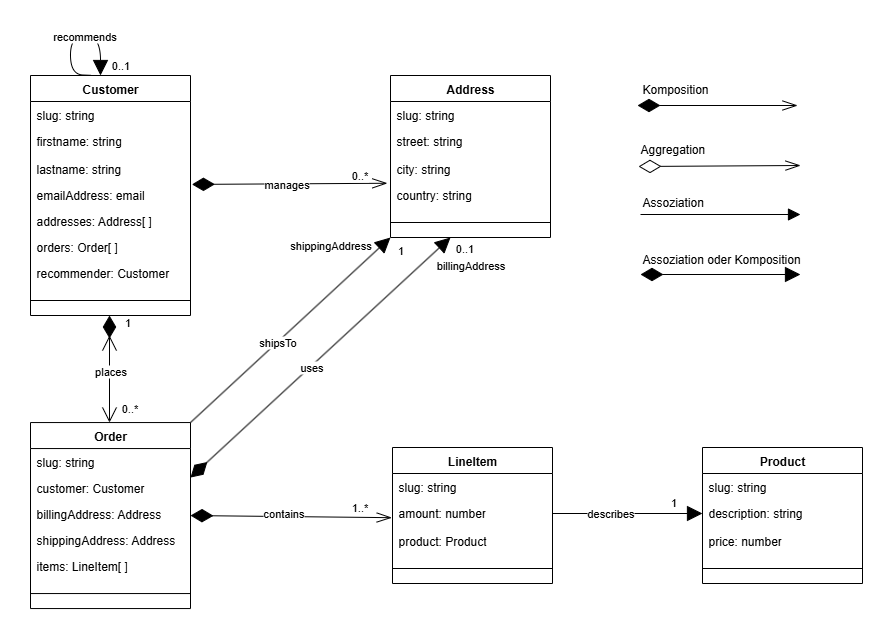
\includegraphics[width=\linewidth]{UML.png}
  \caption{UML-Modell mit Constraints zur Referenzierung und Erstellung}
  \label{fig:uml_modell}
\end{figure}


Für die exemplarische Umsetzung wurde ein Domänenmodell gewählt, das typische Beziehungen aus realen Anwendungsfällen abbildet. Es besteht aus den Typen \texttt{Customer}, \texttt{Order}, \texttt{LineItem}, \texttt{Product} und \texttt{Address} und erfüllt folgende Struktur:

\begin{itemize}
  \item Ein \texttt{Customer} besitzt mehrere \texttt{Order}.
  \item Jede \texttt{Order} enthält eine Liste von \texttt{LineItem}.
  \item Ein \texttt{LineItem} referenziert ein \texttt{Product}.
  \item Zusätzlich besitzt jede Bestellung eine Rechnungs- und eine Lieferadresse vom Typ \texttt{Address}.
\end{itemize}

Das Modell wurde so gewählt, dass es typische Anforderungen an die Referenzierung, Verschachtelung und Wiederverwendung abbildet. Es dient im weiteren Verlauf der Arbeit als durchgehendes Beispiel für das Mapping in Pfadstrukturen, die Analyse von Zyklen sowie die Ableitung von Regeln für das virtuelle Dateisystem und den Language Server.

\subsection{Umsetzung als Datenbankschema}

Das Domänenmodell wird im Based-Schema technisch umgesetzt. Jeder Typ wird im Schema durch eine eigene Struktur mit Präfix, Felddefinitionen und referenziellen Beziehungen abgebildet. Die Feldtypen erlauben eine genaue Definition der Struktur, während über spezielle Schemaeigenschaften zusätzliche Constraints definiert werden können.

Neben der reinen Strukturdefinition werden folgende Mechanismen im Schema verwendet:

\begin{itemize}
  \item \texttt{existsIn} – Einschränkung der Referenz auf zulässige Zieltypen
  \item \texttt{uniqueRef} – Sicherstellung eindeutiger Verweise auf andere Objekte
  \item \texttt{deletePolicy} – Definition, wie sich Löschoperationen auf verknüpfte Objekte auswirken
\end{itemize}

Diese Regeln werden nicht von der Datenbank selbst überprüft, sondern zur Laufzeit durch die Applikation validiert. Dadurch lässt sich das Verhalten der Anwendung vollständig durch das Schema steuern, ohne dass Änderungen im Code erforderlich sind. Dies unterstützt das Ziel einer generischen, domänenunabhängigen Architektur.

\subsection{Analyse und Nutzung zur Laufzeit}

Ein zentrales Element der Lösung ist die Analyse des Schemas beim Start der Anwendung. Dabei wird die Typstruktur rekursiv ausgewertet, um gültige Pfadkombinationen, erlaubte Kindtypen und zyklische Referenzen zu erkennen. Das Ergebnis wird als interne Struktur, z.\,B. \texttt{UriTree}, gespeichert.

Diese Struktur wird verwendet, um das virtuelle Dateisystem aufzubauen. Jeder Pfad im Explorer entspricht einem gültigen Übergang im Typbaum. Die gleiche Struktur dient auch dem Language Server als Grundlage für Funktionen wie Autovervollständigung, Navigation und Validierung. So wird sichergestellt, dass alle Interaktionen im Editor mit dem aktuellen Schema übereinstimmen.

Durch die Analyse zur Laufzeit ist die Lösung vollständig datengetrieben. Neue Typen, Felder oder Regeln können über das Schema ergänzt werden, ohne dass Anpassungen am Quellcode notwendig sind. Damit wird das zentrale Ziel der Arbeit erreicht: eine generische, erweiterbare Umgebung zur Bearbeitung domänenspezifischer Datenmodelle.
